\documentclass{beamer}

%
% Choose how your presentation looks.
%
% For more themes, color themes and font themes, see:
% http://deic.uab.es/~iblanes/beamer_gallery/index_by_theme.html
%
\mode<presentation>
{
  \usetheme{default}      % or try Darmstadt, Madrid, Warsaw, ...
  \usecolortheme{default} % or try albatross, beaver, crane, ...
  \usefonttheme{default}  % or try serif, structurebold, ...
  \setbeamertemplate{navigation symbols}{}
  \setbeamertemplate{caption}[numbered]
  \setbeamertemplate{footline}[page number]
  \setbeamercolor{frametitle}{fg=white}
  \setbeamercolor{footline}{fg=black}
} 

\usepackage[english]{babel}
\usepackage[utf8x]{inputenc}
\usepackage{tikz}
\usepackage{listings}
\usepackage{courier}

\xdefinecolor{darkblue}{rgb}{0.1,0.1,0.7}
\xdefinecolor{dianablue}{rgb}{0.18,0.24,0.31}
\definecolor{commentgreen}{rgb}{0,0.6,0}
\definecolor{stringmauve}{rgb}{0.58,0,0.82}

\lstset{ %
  backgroundcolor=\color{white},      % choose the background color
  basicstyle=\ttfamily\small,         % size of fonts used for the code
  breaklines=true,                    % automatic line breaking only at whitespace
  captionpos=b,                       % sets the caption-position to bottom
  commentstyle=\color{commentgreen},  % comment style
  escapeinside={\%*}{*)},             % if you want to add LaTeX within your code
  keywordstyle=\color{blue},          % keyword style
  stringstyle=\color{stringmauve},    % string literal style
  showstringspaces=false,
  showlines=true
}

\lstdefinelanguage{scala}{
  morekeywords={abstract,case,catch,class,def,%
    do,else,extends,false,final,finally,%
    for,if,implicit,import,match,mixin,%
    new,null,object,override,package,%
    private,protected,requires,return,sealed,%
    super,this,throw,trait,true,try,%
    type,val,var,while,with,yield},
  otherkeywords={=>,<-,<\%,<:,>:,\#,@},
  sensitive=true,
  morecomment=[l]{//},
  morecomment=[n]{/*}{*/},
  morestring=[b]",
  morestring=[b]',
  morestring=[b]"""
}

\title[2016-12-16-overview-of-projects]{Jim Pivarski's Overview of Projects}
\author{Jim Pivarski}
\institute{Princeton -- DIANA}
\date{December 16, 2016}

\begin{document}

\logo{\pgfputat{\pgfxy(0.11, 8)}{\pgfbox[right,base]{\tikz{\filldraw[fill=dianablue, draw=none] (0 cm, 0 cm) rectangle (50 cm, 1 cm);}}}\pgfputat{\pgfxy(0.11, -0.6)}{\pgfbox[right,base]{\tikz{\filldraw[fill=dianablue, draw=none] (0 cm, 0 cm) rectangle (50 cm, 1 cm);}
\includegraphics[height=0.99 cm]{diana-hep-logo.png}\tikz{\filldraw[fill=dianablue, draw=none] (0 cm, 0 cm) rectangle (4.9 cm, 1 cm);}}}}

\begin{frame}
  \titlepage
\end{frame}

\logo{\pgfputat{\pgfxy(0.11, 8)}{\pgfbox[right,base]{\tikz{\filldraw[fill=dianablue, draw=none] (0 cm, 0 cm) rectangle (50 cm, 1 cm);}
\includegraphics[height=1 cm]{diana-hep-logo.png}}}}

% Uncomment these lines for an automatically generated outline.
%\begin{frame}{Outline}
%  \tableofcontents
%\end{frame}

\begin{frame}{My goals}
\vspace{0.6 cm}
\mbox{\hspace{-0.6 cm}\begin{minipage}{1.1\linewidth}
\begin{enumerate}
\item \textcolor{darkblue}{To build bridges between the HEP software ecosystem and the big data ecosystems--- Scientific Python and Hadoop/Spark--- so that HEP data can easily flow between them.}

\begin{itemize}\setlength{\itemsep}{0.1 cm}
\item {\bf Scikit-HEP:} reorganize rootpy, root\_numpy, Ostap and maybe others into a Pythonic layer between HEP and Scientific Python.

\textcolor{gray}{\it with Eduardo, David, Noel Dawe, Vanya Belyaev, and Sasha Mazurov}

\item {\bf root4j/spark-root:} pure-Java ROOT I/O for Spark integration.

\textcolor{gray}{\it with Viktor Khristenko, for Oliver Gutsche and Matteo Cremonesi}

\item {\bf Scope:} NoSQL database/server for interactive analysis.

\textcolor{gray}{\it with Jin Chang and Igor Mandrichenko}
\end{itemize}

\item \textcolor{darkblue}{To build computational engines in those big data ecosystems that allow us to perform HEP-style analyses when we get there.}

\begin{itemize}\setlength{\itemsep}{0.1 cm}
\item {\bf Histogrammar:} functional interface to aggregation.

\textcolor{gray}{\it with Alexey Svyatkovskiy for Oliver Gutsche and Matteo Cremonesi}

\item {\bf Femtocode:} query language for Scope and Spark DataFrames.

\textcolor{gray}{\it just me, for Jin Chang and Igor Mandrichenko}
\end{itemize}
\end{enumerate}
\end{minipage}}
\end{frame}

\begin{frame}{They're all connected}
\begin{center}
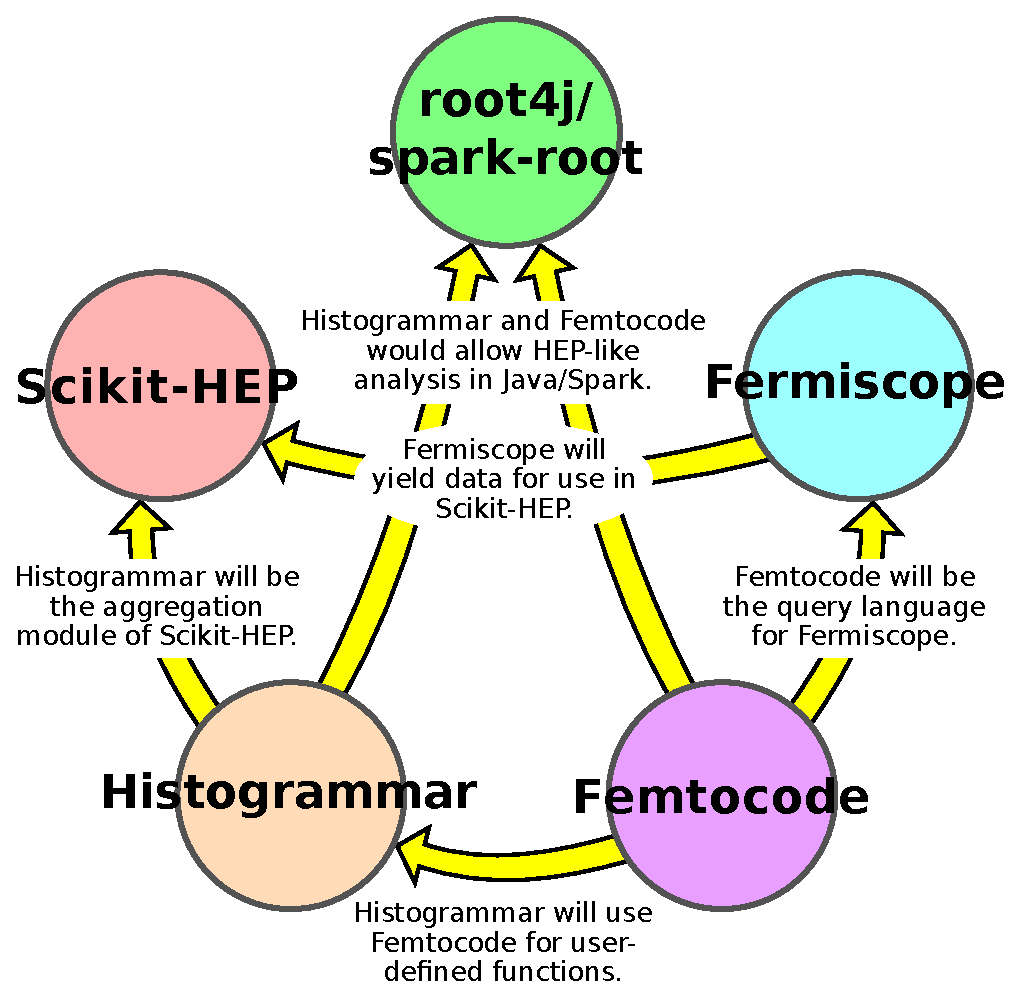
\includegraphics[width=0.78\linewidth]{relationships.pdf}
\end{center}
\end{frame}

\begin{frame}{Meta-strategy}
\vspace{0.25 cm}
\begin{itemize}
\item Diverse suite of projects with interconnections:
\begin{itemize}
\item Not everything has to work, but they're all better if they do.
\item If a competitor succeeds in some area, don't fight them. Concentrate on the others while the connection to successful projects provides an implicit incentive to grow later.
\end{itemize}

\item Focusing on building developer communities before user communities.
\begin{itemize}
\item Aiming for 1--2 users of each project once it's minimally useful.
\item But I'm trying to bring in as many developers as there are use-cases, to each concentrate on their favorite part.
\item This includes developers outside of HEP (if possible).
\item Planning on using focus groups to guide design, rather than just reacting with release-early-release-often.
\end{itemize}
\end{itemize}
\end{frame}

\begin{frame}{Goal}
\textcolor{darkblue}{Goal: widely used code and some publications.}

\vspace{0.25 cm}
Not much to show yet:

\begin{itemize}
\item Histogrammar is user-ready but its adoption is slow. People in HEP and industry are excited when they see it, but never follow up with applications. Missed ROOT release date because ROOT is not ready to include Python subpackages. Will target Scikit-HEP instead. \textcolor{gray}{(And possibly fitting a C++ Histogrammar into Enrico Guiraud's functional chains.)}

\item All other projects are too early to judge.

\item Missed round of HEP-computing conference deadlines because they're early in the year and I wasn't ready back then. Gearing up for next year's cycle.
\end{itemize}
\end{frame}



\end{document}
